\documentclass{article}

\usepackage[english]{babel}

% Set page size and margins
\usepackage[a4paper,top=2cm,bottom=2cm,left=3cm,right=3cm,marginparwidth=1.75cm]{geometry}

% Useful packages
\usepackage{amsmath}
\usepackage{graphicx}
\usepackage[colorlinks=true, allcolors=blue]{hyperref}
\usepackage{color}
\usepackage{minted}
\usepackage{tikz}
\usepackage{placeins}
\usepackage{float}
\usepackage[utf8]{inputenc}
\usepackage[T1]{fontenc}
\usepackage{fullpage}
%\usepackage[numbers]{natbib}
\usepackage{minted}
\usepackage{amsmath,amssymb,amsfonts}
\usepackage{algorithmic}
\usepackage{graphicx}
\usepackage{textcomp}
\usepackage{placeins}
\usepackage{tabularx}
\usepackage{svg}

\usepackage[style=ieee]{biblatex}
\addbibresource{sample.bib}

%\setkeys{Gin}{width=\linewidth,totalheight=\textheight,keepaspectratio}

% Credit to Steven B. Segletes on StackExchange
% https://tex.stackexchange.com/a/265804

\usepackage[most]{tcolorbox}
\definecolor{block-gray}{gray}{0.85}
\newtcolorbox{myquote}{colback=block-gray,grow to right by=-10mm,grow to left by=-10mm, boxrule=0pt,boxsep=0pt,breakable}
\makeatletter
\def\quoteparse{\@ifnextchar`{}{\singlequote}}
\makeatother
\def\singlequote#1`{\texttt{#1}\quoteON}
\def\doublequote#1``{\texttt{#1}\quoteON}
\long\def\triplequote#1```{\begin{myquote}\parskip 1ex#1\end{myquote}\quoteON}
\def\quoteON{\catcode``=\active}
\def\quoteOFF{\catcode``=12}
\quoteON
\def`{\quoteOFF \quoteparse}
\quoteOFF

%from https://blogs.gnome.org/muelli/2011/04/perfectly-scale-an-image-to-the-rest-of-a-page-with-latex/
\newlength{\textundbildtextheight}
\newcommand{\textundbild}[2]{
\settototalheight\textundbildtextheight{\vbox{#1}}
#1
\vfill
\begin{center}
\includegraphics[width=\textwidth,keepaspectratio=true,height=\textheight-\the\textundbildtextheight]{#2}
\end{center}
\vfill
}



% Thanks to leandriis on StackOverflow for this formatting https://tex.stackexchange.com/a/533609
\usetikzlibrary{positioning,shapes.misc, shapes.geometric, arrows}


\tikzstyle{arrow} = [thick,->,>=stealth]
\tikzstyle{tCircle} = [circle, draw=black, align=center, minimum width=2cm]
\tikzstyle{tRoundRect} = [rounded rectangle, draw=black, align=center, minimum width=3cm, minimum height=1cm, text centered]
\tikzstyle{tRect} = [rectangle, draw=black, align=center, minimum width=3cm, minimum height=1cm, text centered]

\title{%
    Evaluating Effective Interventions on Individuals in Infelicitous Eventualities\\
    \large An initial proposal report discussing a pair of Causal Inference tasks\\
    and a proposed approach for solving these two problems.
    }
\author{2100816}
\begin{document}
\maketitle
\quoteON

\begin{table}[h]
    \centering
    \begin{tabular}{ll}
        Registration number: & \textcolor{red}{2100816}\\
        Project: & \textcolor{red}{Causal inference}\\
        Link to GitHub: & \url{https://github.com/11BelowStudio/ce888}\\
    \end{tabular}
\end{table}



\begin{table}[h]
    \centering
    \begin{tabular}{lc}
        Executive summary (max.\ 250 words) & \textcolor{red}{96}\\
        Introduction (max.\ 600 words) & \textcolor{red}{599}\\
        Data (max.\ 500 words/dataset) & \textcolor{red}{\textit{(538 + 459)} = 997}\\
        Methodology (max.\ 600 words) & \textcolor{red}{635}\\
        Conclusions (max.\ 500 words) & \textcolor{red}{473}\\
        \hline
        Total word count & \textcolor{red}{2800}\\
    \end{tabular}
    \caption{Word counts for each section.}
\end{table}

\tableofcontents

\clearpage



\begin{abstract}
This document is the formal proposal document for a causal inference investigation
into the the IHDP\cite{Gross1993} \cite{BROOKSGUNN1992350} and JOBS\cite{JOBS_LaLonde}\cite{JOBS2}\cite{ASMITH2005305} datasets.

This document introduces the context for the problem,
discusses some findings from an initial exploration of these datasets
(providing visualizations of these datasets to supplement this),
and provides a proposed methodology for how the next stages of this investigation
shall be achieved.

The preliminary investigation has identified some potential roadblocks for the latter parts of the
investigation, which could pose a few barriers to the potential for meaningful conclusions to be
reached, however, these are not insurmountable.
\end{abstract}


\section{Introduction}

This project involves two datasets: the Infant Health and Development Program (`IHDP`)\cite{Gross1993}\cite{BROOKSGUNN1992350} and `JOBS`\cite{JOBS_LaLonde}\cite{JOBS2}\cite{ASMITH2005305}.


Both of these datasets contain information about individuals (`x`),
whether or not the individuals received some 'treatment' (`t`),
and a `y` outcome for the individuals. The task I have been given for these datasets
is to find the causal relationships within these datasets, to assess whether or not
the treatments (`t`) given to the individuals have had any effect on the outcomes (`y`).


As discussed by Hill and Stuart, 'Causal Inference' is the term used to refer to
the overall task of investigating how a 'causal variable' may influence an 'outcome',
and what conclusions can be drawn from that. There is a particular interest
in trying to predict 'the outcomes that could manifest given exposure to each of
a set of treatment conditions', allowing one to perform 'comparisons between
these 'potential outcomes''\cite{HILL2015255}. This act has practical applications
that serve genuine benefits besides the existential flex of predicting an
alternative timeline, for example, Glass et al mention how this act of identifying
causal relationships has formed the backbone of public health policy and modern medical
practice, and emphasize the importance of using causal inference to establish
the effects of interventions, not just underlying causes, to allow meaningful
interventions to be made as and when necessary\cite{Glass2013}.
This relates to the concept of Causal Decision-Making, which, by itself, does not
need the counterfactuals and causal effects to be calculated (only needing
an estimator of `y` given `x` and `t`). Fernández-Loría and Provost do stress
the importance of not overcomplicating that particular task through
unnecessarily introducing counterfactuals, however, they do point out that
causal inference is vital for evaluating the success of these
causal decisions\cite{fernandezloria2021causal}.


In context of the `IHDP` and `JOBS` datasets; `IHDP` concerns the cognitive development
of prematurely-born children, with an intervention in the form of additional support being
given to the families in the control group, with the intent being to, as the name implies,
support the health and development of these infants, throughout their
childhoods\cite{Gross1993}\cite{BROOKSGUNN1992350}. This intervention could provide many
benefits to the parents and the child besides being able to score high on cognitive
ability tests (the subset of the `IHDP` dataset I have access to for this project only
has a cognitive ability test result score as a `y` outcome though), however, if
a meaningful result for the intervention cannot be demonstrated, it is unlikely
that resources would be allocated to allow this intervention to be sustained long-term,
for more individuals. Furthermore, if it is found to be ineffective, that could be
seen as a motivation to find other potential interventions that may turn out to be more
effective (and worthy of being used in the long term).


`JOBS`, on the other hand, concerns the effect of a support program on helping individuals
who are unemployed to gain employment (with a rather large control group consisting
of individuals who were not on this support program)\cite{JOBS_LaLonde}\cite{JOBS2}\cite{ASMITH2005305}.
This dataset arguably does have a somewhat uninformative `y` value, just like `IHDP`,
as this `y` is merely a binary value (employed or unemployed), regardless of the
variety of employment (whether that 'employment' be in the form of a stable, well-paid job,
or underemployed without any job security). However, just like in the situation of
`IHDP`, if the treatment doesn't have any positive effect on whether or not an individual
can successfully gain employment (especially when considering the employment outcomes for
other, similar, individuals who were not receiving this additional support),
this particular support, being unfit for purpose, would need to be replaced by a more
effective intervention.

\section{Data}


\subsection{IHDP - The Infant Health Development Program}

\FloatBarrier

\quoteON

`IHDP` consists of real data regarding the effects of providing additional support to the
families who had premature babies on the development of aforementioned babies, measured
through the means of IQ tests\cite{Gross1993}\cite{BROOKSGUNN1992350}. The version of this
dataset used in this task contains factual and (simulated) counterfactual data; however,
I shall only use the counterfactual data for evaluating fully trained models.


This dataset concerns a population of 750 individuals, all of whom have 25 \texttt{x} values,
a \texttt{t} value indicating whether they were in the treatment/control group, as well as
a factual \texttt{yf} value (indicating the true \texttt{y} value recorded from that individual
during the experiment), and a counterfactual \texttt{ycf} value (derived via a simulation,
simulating the outcome for that individual if they were in the opposite treatment/control group to
the group they actually were in). There is also an \texttt{ite} value, providing the individual
treatment effect for the individuals. The \texttt{y} values are continuous values.


A visualization of this dataset can be seen in \ref{fig:ihdpgraphs} (along with an overview
of the factual data within \ref{fig:ihdpfact}, and of the counterfactual data within \ref{fig:ihdpcf}).


Of the 25 'x' values, 6 of them are in a continuous range, whilst the other 19 are binary.
One of these non-binary 'x' values, \texttt{x3} , appears to be limited to one of four discrete
values; however, as I have been unable to conclusively find out what \texttt{x3} truly means,
and as that means it could possibly have a different value, I shall not normalize that into
discrete values, to allow leeway for potential future data, which may have a different value.


\begin{figure}[htb]
\centering
    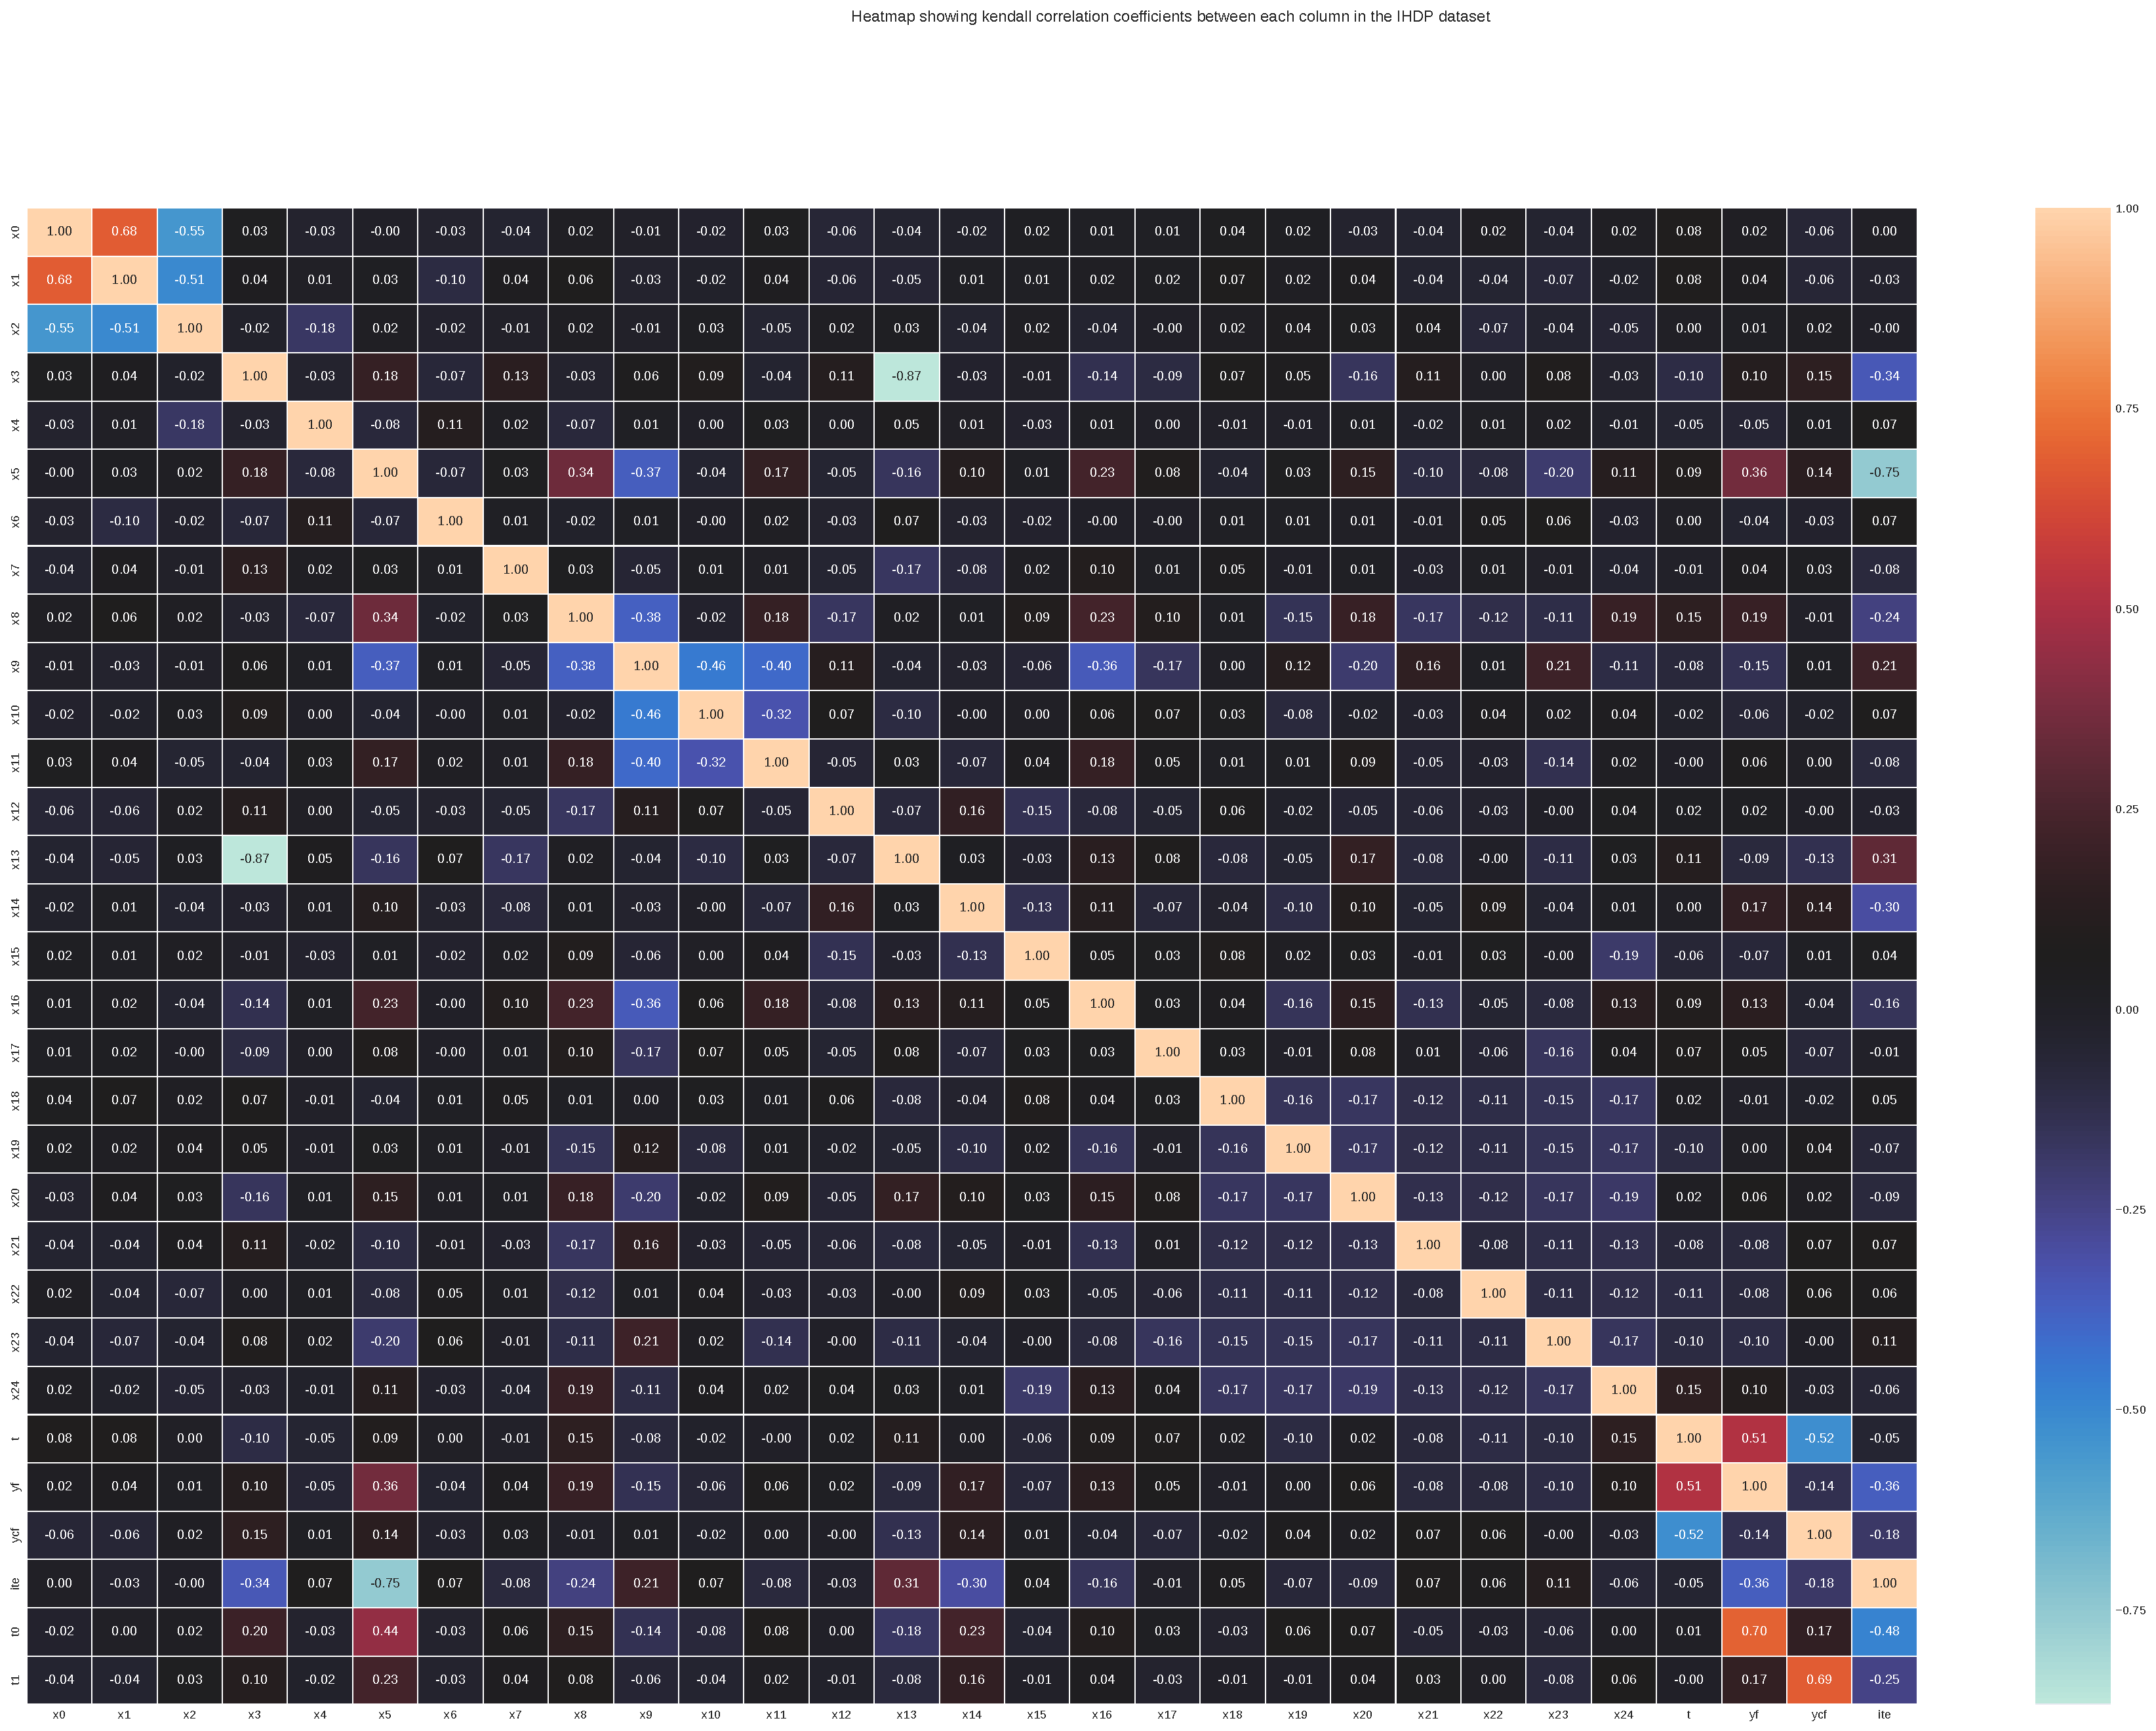
\includegraphics[width=0.9\textwidth]{project/data/ihdp_heatmap.pdf}
    \caption{
        \label{fig:ihdp_correlation}Correlation heatmap for the IHDP dataset
    }
    \small{
        This annotated heatmap shows the correlation coefficients for the values in each
        column of the IHDP dataset (along with additional \texttt{t0} and \texttt{t1} columns). 
        \texttt{t0} contains the \texttt{y} values for each individual for the case
        where \texttt{t=0}, and vice versa for \texttt{t1} (with these columns being included
        for ease of looking at overall treatment/control outcomes).
        
        There isn't much clear correlation between the values of each column in this dataset,
        barring a few outliers.
        
        There is a rather strong positive correlation between \texttt{t} and \texttt{yf} (with a
        slightly stronger negative \texttt{t}/\texttt{ycf} correlation), indicating that
        being in the treatment group correlates to a higher \texttt{y}, but whether or not this
        is due to causation does need to be investigated further.
    }
\end{figure}


Figure \ref{fig:ihdp_correlation} indicates a lack of much correlation in this dataset,
barring a few notably higher correlations.

There is a rather strong negative
correlation between \texttt{x5} and \texttt{ite} (and, in extension,
\texttt{x5}'s relation to \texttt{t0} and \texttt{t1}), to see if this correlation
truly indicates whether a higher \texttt{x5} can cause the treatment to have an
unintended effect. This correlation is also illustrated in Figure \ref{fig:ihdpgraphs},
showing this strong downward trend. However, looking at the \texttt{x5}
data in Figure \ref{fig:ihdpfact}, we can see some individuals with high \texttt{x5}
values in the untreated group achieved rather high \texttt{yf} scores (but only with a \texttt{x5}
and \texttt{yf} correlation of 0.36), so one could argue that the negative ITE correlation
could be due to the counterfactual simulation not allowing similar \texttt{ycf}
values to be reached (with counterfactuals illustrated in Figure \ref{fig:ihdpcf}).

Other notable correlations include a strong negative correlation of -0.87 between \texttt{x3} and \texttt{x13}, indicating a potential causal link. A weaker positive correlation (0.68) is present
between `x0` and `x1` (with slightly weaker negative correlations between those and `x2`).
These correlations could be a sign of causation between these variables,
or they could be an indicator of an external confounder, or perhaps neither, which justifies
some further investigation.

\subsubsection{The Causal Questions}

\begin{enumerate}
\item To what extent does each \texttt{x} predict \texttt{y}?
\item To what extent does \texttt{t} predict \texttt{y}?
\item To what extent do the \texttt{x} values predict each other?
\item To what extent do the \texttt{x} values predict the \texttt{ite} values?
\end{enumerate}

\subsubsection{Metrics to use}

As this dataset contains full counterfactual/ITE data, I am able to use Precision in
Estimation of Heterogenous Effect ($\epsilon PEHE$) and Average Treatment Effect ($\epsilon ATE$)
in order to measure the correctness of the learner's estimations of individual treatment
effects\cite{CE888_causal}.


\FloatBarrier

\subsection{JOBS}
\FloatBarrier
\quoteON

`JOBS` contains data about 3212 jobseekers (`x`), whether or not they
received support to get a job (`t`), and whether or not they were successful in
gaining employment (`y`, with a value of 0 or 1)\cite{JOBS_LaLonde}\cite{JOBS2}\cite{ASMITH2005305}.
There is no counterfactual data within this dataset, and the dataset is derived from experimental
and observational data (with this being denoted by `e`).
This dataset is incredibly unbalanced, with only 297 individuals being in the treatment group,
and only 482 individuals with `y=0`, which will pose some problems with regards to avoiding
overfitting.

Furthermore, many of the `x` values are binary, with the non-binary `x` values having particularly
extreme ranges (requiring the use of a log scale to graph those appropriately, as can be seen in Figure \ref{fig:jobsgraphs}),
heavily necessitating some normalization before training is attempted. 

\begin{figure}[ht]
\centering
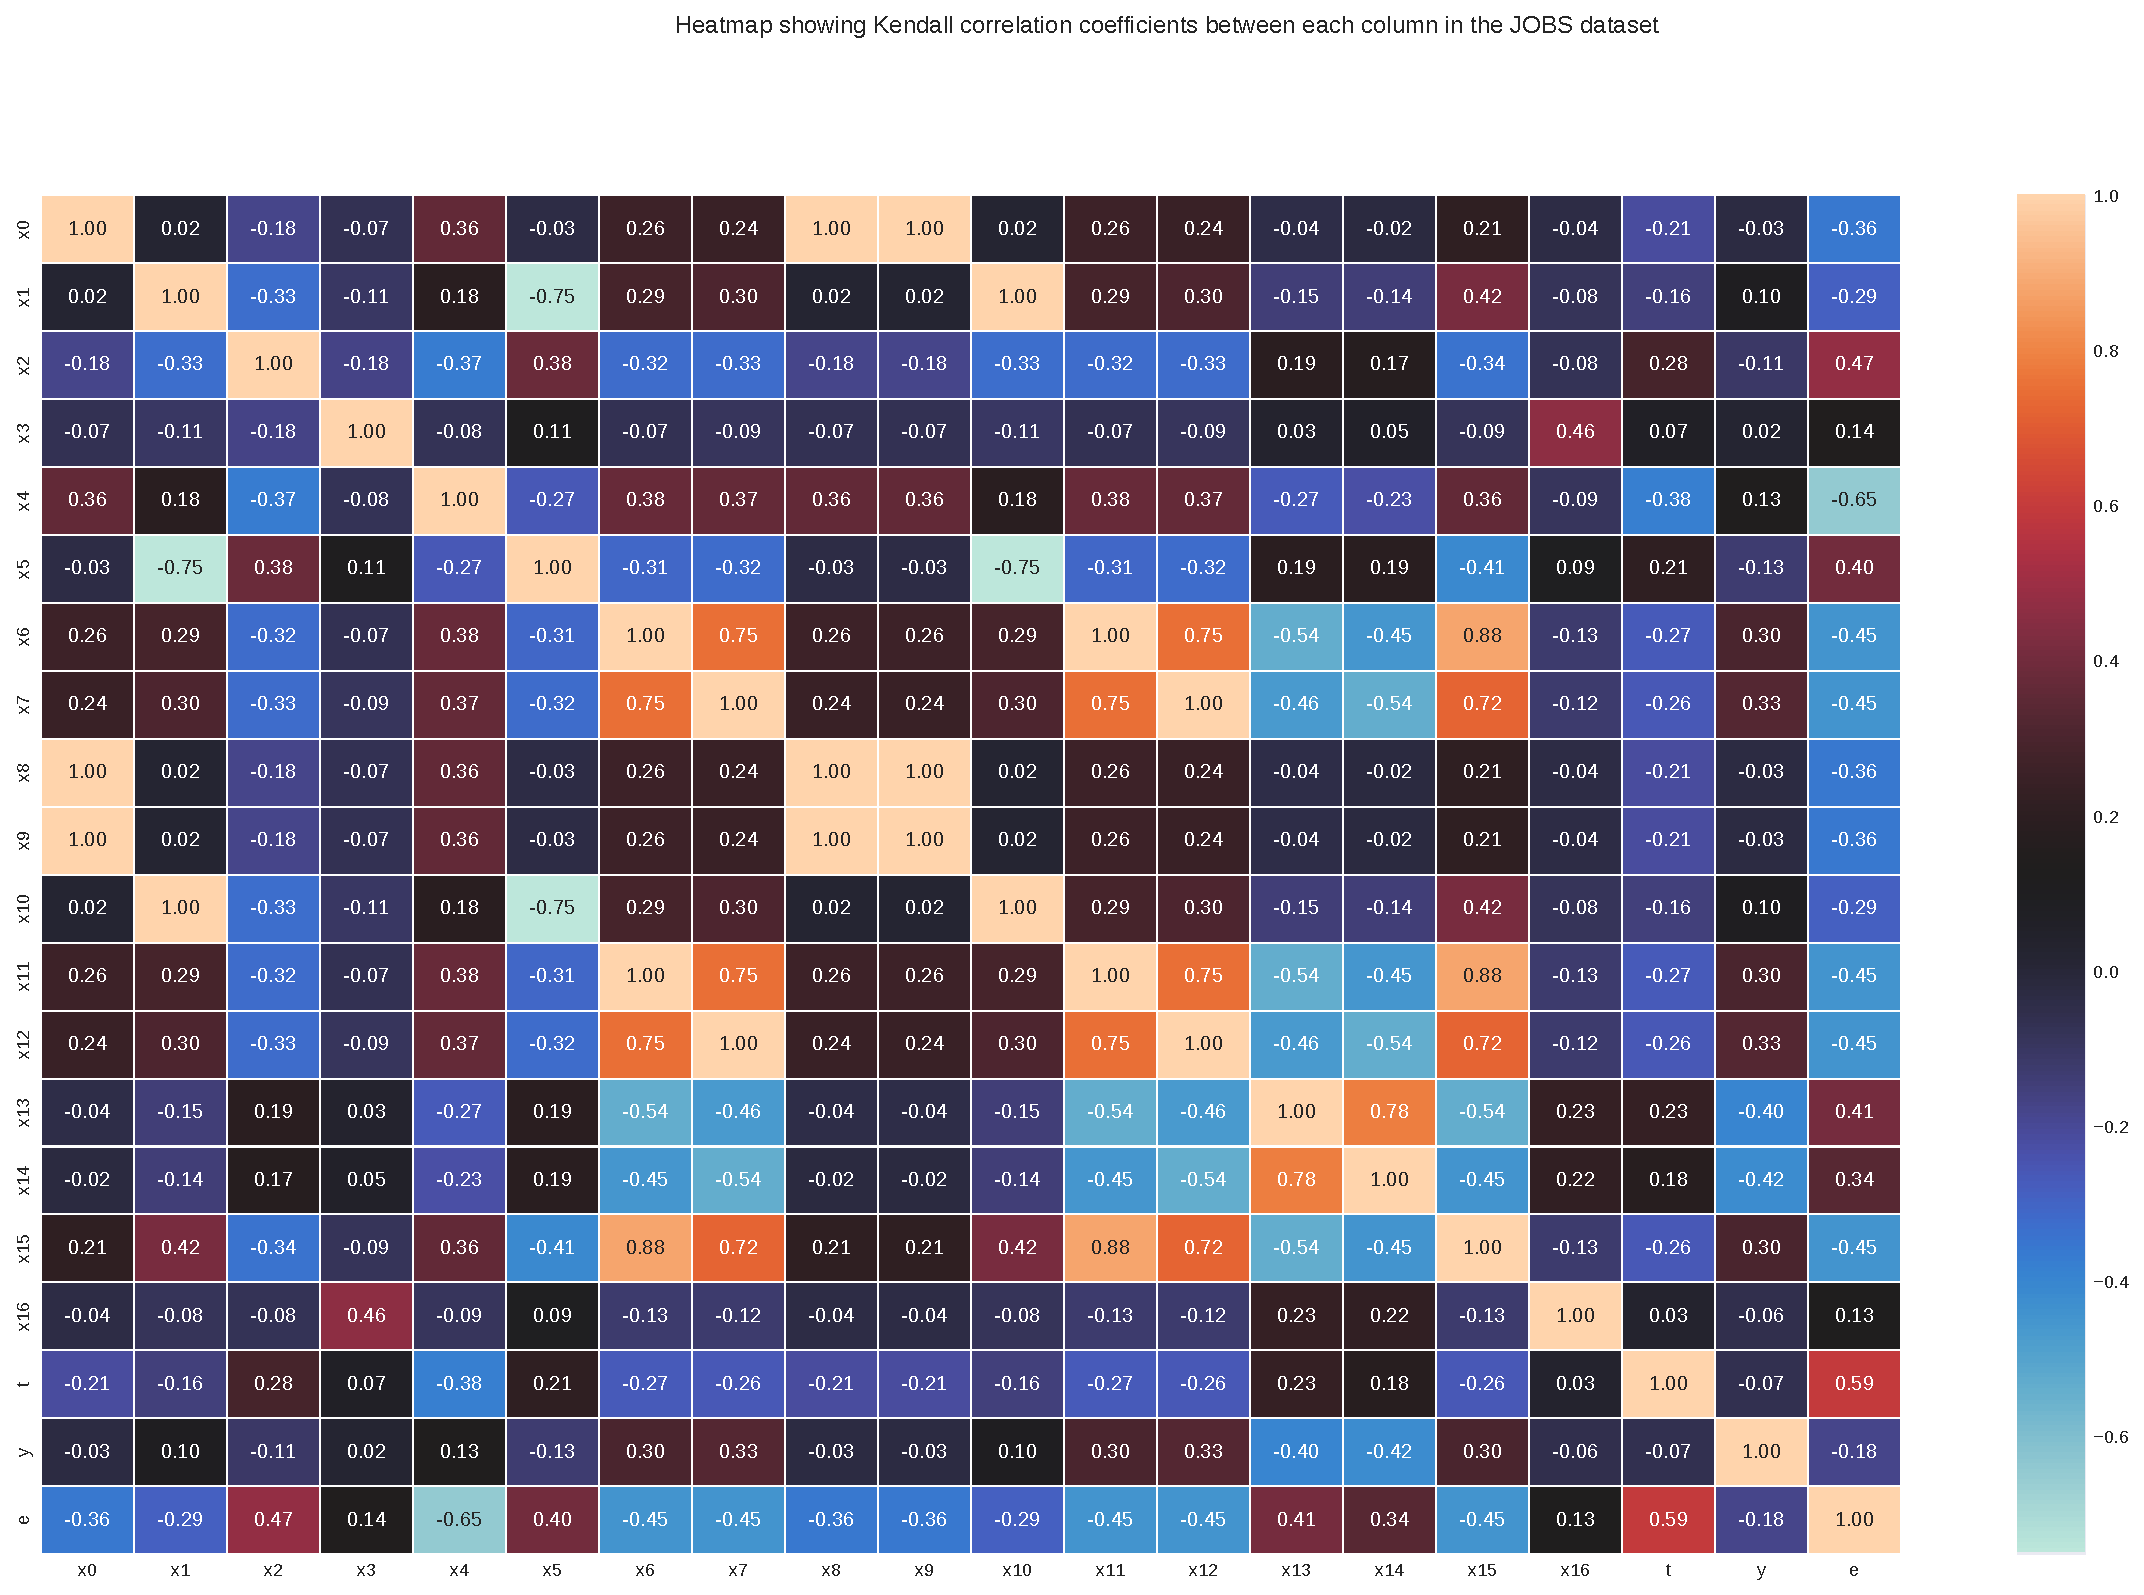
\includegraphics[width=0.9\textwidth]{project/data/jobs_heatmap.pdf}
\caption{\label{fig:jobs_correlation}Correlation heatmap for the JOBS dataset}
\end{figure}

Looking at the correlation heatmap for `JOBS` in figure \ref{fig:jobs_correlation},
we can see that there is significant correlation within the dataset,
with perfect positive correlation between `x0`,`x8`, and `x9`.
`x1` and `x10` also have perfect positive correlation, along with
`x11` and `x6`, and again with `x12` and `x7` (with many other sets of
variables having imperfect yet rather high magnitudes of correlation).
Upon looking at figure \ref{fig:jobsgraphs}, these identified areas
of perfect correlation aren't particularly unbalanced, but all of them
are `x` values where `x` is in a range, instead of being binary.
Interestingly, there isn't any strong correlation between `y` and
any other variable, whilst `t` and `y` have a weak negative correlation of
$-0.07$, suggesting that the treatment doesn't have any bearing on the
overall outcome. This implies the presence of some confounder having
a stronger bearing on the `y` value, or that, if there is a causal
relation between `x` and `y`, a combination of `x` values is what
indicates the outcome.


\subsubsection{The Causal Questions}

\begin{enumerate}
\item Does `t` have any meaningful effect on `y`?
\item Do any `x` values meaningfully predict `y`? Do `t` or the other `x` values have an impact on this?
\item Do any `x` values have a causal interrelationship?
\item How can we measure the individual treatment effects due to a lack of counterfactuals?
\end{enumerate}

\subsubsection{Metrics to use}

Due to the binary nature of `y`, it is possible to approach some aspects of this dataset
from the perspective of a classification rather than a regression approach, meaning that
we could use classification-based metrics, such as logistical loss to estimate the accuracy
of `y` estimators.
\cite{sklearnmetricsloglossscikitlearn102documentation}

For measuring any Conditional Average Treatment Effects, the lack of counterfactuals
requires either a Policy Loss metric (as explained in \cite{CE888_project_causality}),
or a 'Average Treatment Effect on treated' metric\cite{CE888_causal}.
However, as there are very few individuals who were treated, attempting to use the latter to
assess performance on the full dataset is very likely to result in it being overfit.
Therefore, Policy Loss shall have to be used instead.

\FloatBarrier


\section{Methodology}

\subsection{Preparing the learners}

\FloatBarrier

\quoteON

Before starting any training of the machine learners, I shall split the datasets into a learning
set (to use in training via K-fold cross validation) and a validation set.

Furthermore, for sake of consistency, I shall use an RNG instance with a seed of 42 for the
notebook, allowing reproducible results.

I shall use all of the counterfactual data of `IHDP`, along with ~10\% of the factual data
(aiming to stratify based on treatment/control and the ITE counterfactual data) as its validation set,
leaving the remaining factual data available for k-fold cross validation training.

For the JOBS dataset, I shall use 20\% of the full data as the validation set (20\% of treatment/control,
aiming to stratify based on the outcomes), leaving the remaining 80\% for training/testing.

When performing the testing, I shall be using scikit-learn's pipeline API, using pipelines with the structure
explained in \ref{fig:pipeline}, for ease of re-running experiments, and using `GridSearchCV`
to perform hyper-parameter tuning during K-fold training.

\begin{figure}[htb]
    \centering
    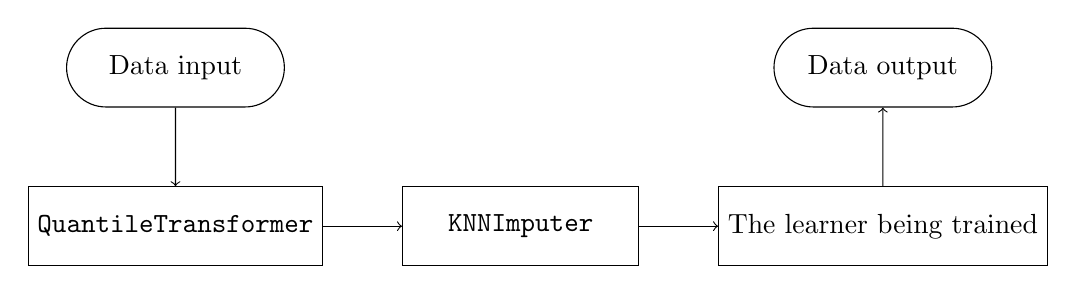
\begin{tikzpicture}
        \node[tRoundRect] (Start) {Data input};
        \node[tRect] (QTrans) [below =of Start] {\texttt{QuantileTransformer}} edge [<-] (Start);
        \node[tRect] (KNNImp) [right =of QTrans] {\texttt{KNNImputer}} edge [<-] (QTrans);
        \node[tRect] (Learner) [right =of KNNImp] {The learner being trained} edge [<-] (KNNImp);
        \node[tRoundRect] (Output) [above =of Learner] {Data output} edge [<-] (Learner);
    \end{tikzpicture}
    \caption{\label{fig:pipeline}Structure for the pipelines to be used for training}
\end{figure}

\FloatBarrier

\subsection{Simple Learners}

\quoteON

To obtain feature importances, I will attempt training a `RandomForestRegressor`,
an `ARDRegressor`, and a couple of `AdaBoostRegressor`s (consisting of the aforementioned
other regressors) to predict the `y` outcomes for individuals given their `x` attributes
and whether or not they have been treated (using `GridSearchCV` to handle hyper-parameter
optimization). The `RandomForestRegressor` shall be used due to how it conveniently provides a
method for returning feature importances @\cite{sklearnensembleRandomForestRegressorscikitlearn102documentation}.
Obtaining these importances is slightly
more convoluted with the `ARDRegressor`, however, there is a workaround to obtaining these.
Despite the necessity of this workaround, the `ARDRegressor`, being a Relevance Vector Machine,
aims to perform regression by trying to weight the inputs based on evidence maximization,
in turn indirectly providing feature importances, without relying as much on a random seed.
\cite{Fletcher10relevancevector}\cite{sklearnlinearmodelARDRegressionscikitlearn102documentation}
The `AdaBoostRegressor` is an extension of these; effectively applying multiple instances of
the same regressor to the problem, weighting each one appropriately to catch the cases which
were missed by the previous regressors within the ensemble.
\cite{sklearnensembleAdaBoostRegressorscikitlearn102documentation}

The classification accuracy for this stage shall be assessed via `r2` scores,
comparing the predicted `y` for the individual (from their `x` and `t`) to the factual `y` value.
`r2` has been chosen due to how it provides a clear indicator of how good the estimator is compared
to returning the expected `y` value (on top of how close the estimator is to returning 'true' `y`
values), clearly indicating how good the predictions are.
\cite{sklearnmetricsr2scorescikitlearn102documentation}


\subsection{Propensity Score re-weighting}

\quoteON

Similar to the 'Simple Learners' stage, I shall try using the identified classification models
to predict propensity scores for each dataset (by aiming to predict `t` given `x`), and then
using the identified 'best' classifier to predict what class they will be in (and giving that
to the Inverse Propensity Score function to produce the actual sample weights).
Unfortunately, due to the `ARDRegressor` not supporting sample weights, I will need
to replace it with a standard `BayesianRidge` regressor for this, but it has a similar end result
\cite{sklearnlinearmodelBayesianRidgescikitlearn102documentation}.

I will then repeat the process outlined in 'Simple Learners' with these weighted models,
and compare the results of the learners with weighted samples to the performance of the
unweighted learners. 

\subsection{Advanced CATE estimators}

\quoteON

I shall attempt to compare the performances of the 
`XLearner`\cite{econmlmetalearnersXLearnereconml0130documentation},
`CausalForestDML`\cite{econmldmlCausalForestDMLeconml0130documentation},
and `ForestDRLearner`\cite{econmldrForestDRLearnereconml0130documentation}
CATE models, implemented as part of EconML\cite{econml},
giving them the 'best' trained propensity and y-prediction models,
and evaluating their performances on predicting treatment effects.

Each of these models come from different categories of CATE model, thereby allowing
different aspects of the conditional treatment effect to be modelled.

During training, I shall evaluate the performances of these models on their 'policy risk'
scores of the factual dataset (using the equation specified in the assignment brief)
\cite{CE888_project_causality}. After training is done, I can evaluate the overall
performance of the `IHDP` model via Precision in Estimated Heterogenous Effects,
due to the presence of counterfactuals (which will not be possible for `JOBS`)\cite{CE888_causal}.

\section{Conclusions}

This project seems somewhat feasible. The `IHDP` dataset looks like it is less likely to cause
problems later on, as, due to it containing data for individual treatment effects and
counterfactuals, it doesn't suffer significantly from an imbalance between treatment and
control groups (although the factual data, which I need to use for testing, does),
and this does permit some slightly easier evaluation of accuracy predictions after training is
complete. However, from a more cynical perspective, that arguably does prompt the question
of whether or not the findings I can derive from this will be of much practical use,
as the presence of counterfactuals suggests that someone else already has fully analysed
this dataset to the point of being able to fully simulate it, so, if a client were to
realistically request an analysis of this particular dataset, one could, in theory,
simply refer to existing literature, as this dataset isn't devoid of prior analysis.

However, the JOBS dataset could pose some significant problems. Besides the lack of
counterfactuals, the massive imbalance between the sizes of the treatment and control
groups compounds the existing imbalances between the quantities of individuals with each
outcome (and for each `x` value). Of course, estimating the effect of a treatment 
(and what the effect would have been
without the treatment) is one of the key tasks in causal inference, and it's generally
physically impossible to get counterfactual data without having already analysed the
factual data enough to accurately simulate the counterfactuals (unless, of course,
one manages to somehow prove the many-worlds theorem and find the correct other world
with the perfect counterfactuals available, but, if the necessary preconditions for that
were to be met, this current task would probably be the least of one's concerns),
so the lack of counterfactuals in `JOBS` is understandable. However, the limited
treatment group data (presumably due to the criteria which individuals had to meet
in order to be allowed into the treatment group, as explained in \cite{ASMITH2005305})
is likely to pose problems, especially if the predictor is provided with unseen data
for an individual who would not have been included in the treatment group, and
is expected to predict what the outcome would have been if they had received
treatment (due to a lack of similar individuals in the treatment group to
compare that individual to).

To conclude, I do not anticipate that any truly meaningful conclusions will be
reached from my analysis of these datasets, but it is by no means impossible for
that to happen, assuming that I am actually approaching this task from the
correct angle. That said, I do not see merit in promising things which I
know I cannot guarantee, so, whilst I cannot formally promise the meaningful
outcome, I can at least promise to attempt delivering such an outcome
within any future analysis of these datasets.


\appendix
\section{Appendix: The visualizations of the datasets}\label{appendix:graphs}

These figures are located in this appendix simply because they're too large for \LaTeX to neatly
insert them within the main content of this report in a location that makes sense.

\subsection{IHDP dataset visualizations}


Here are the graphs for the IHDP dataset.

\FloatBarrier

\begin{figure}[H]
    \centering
    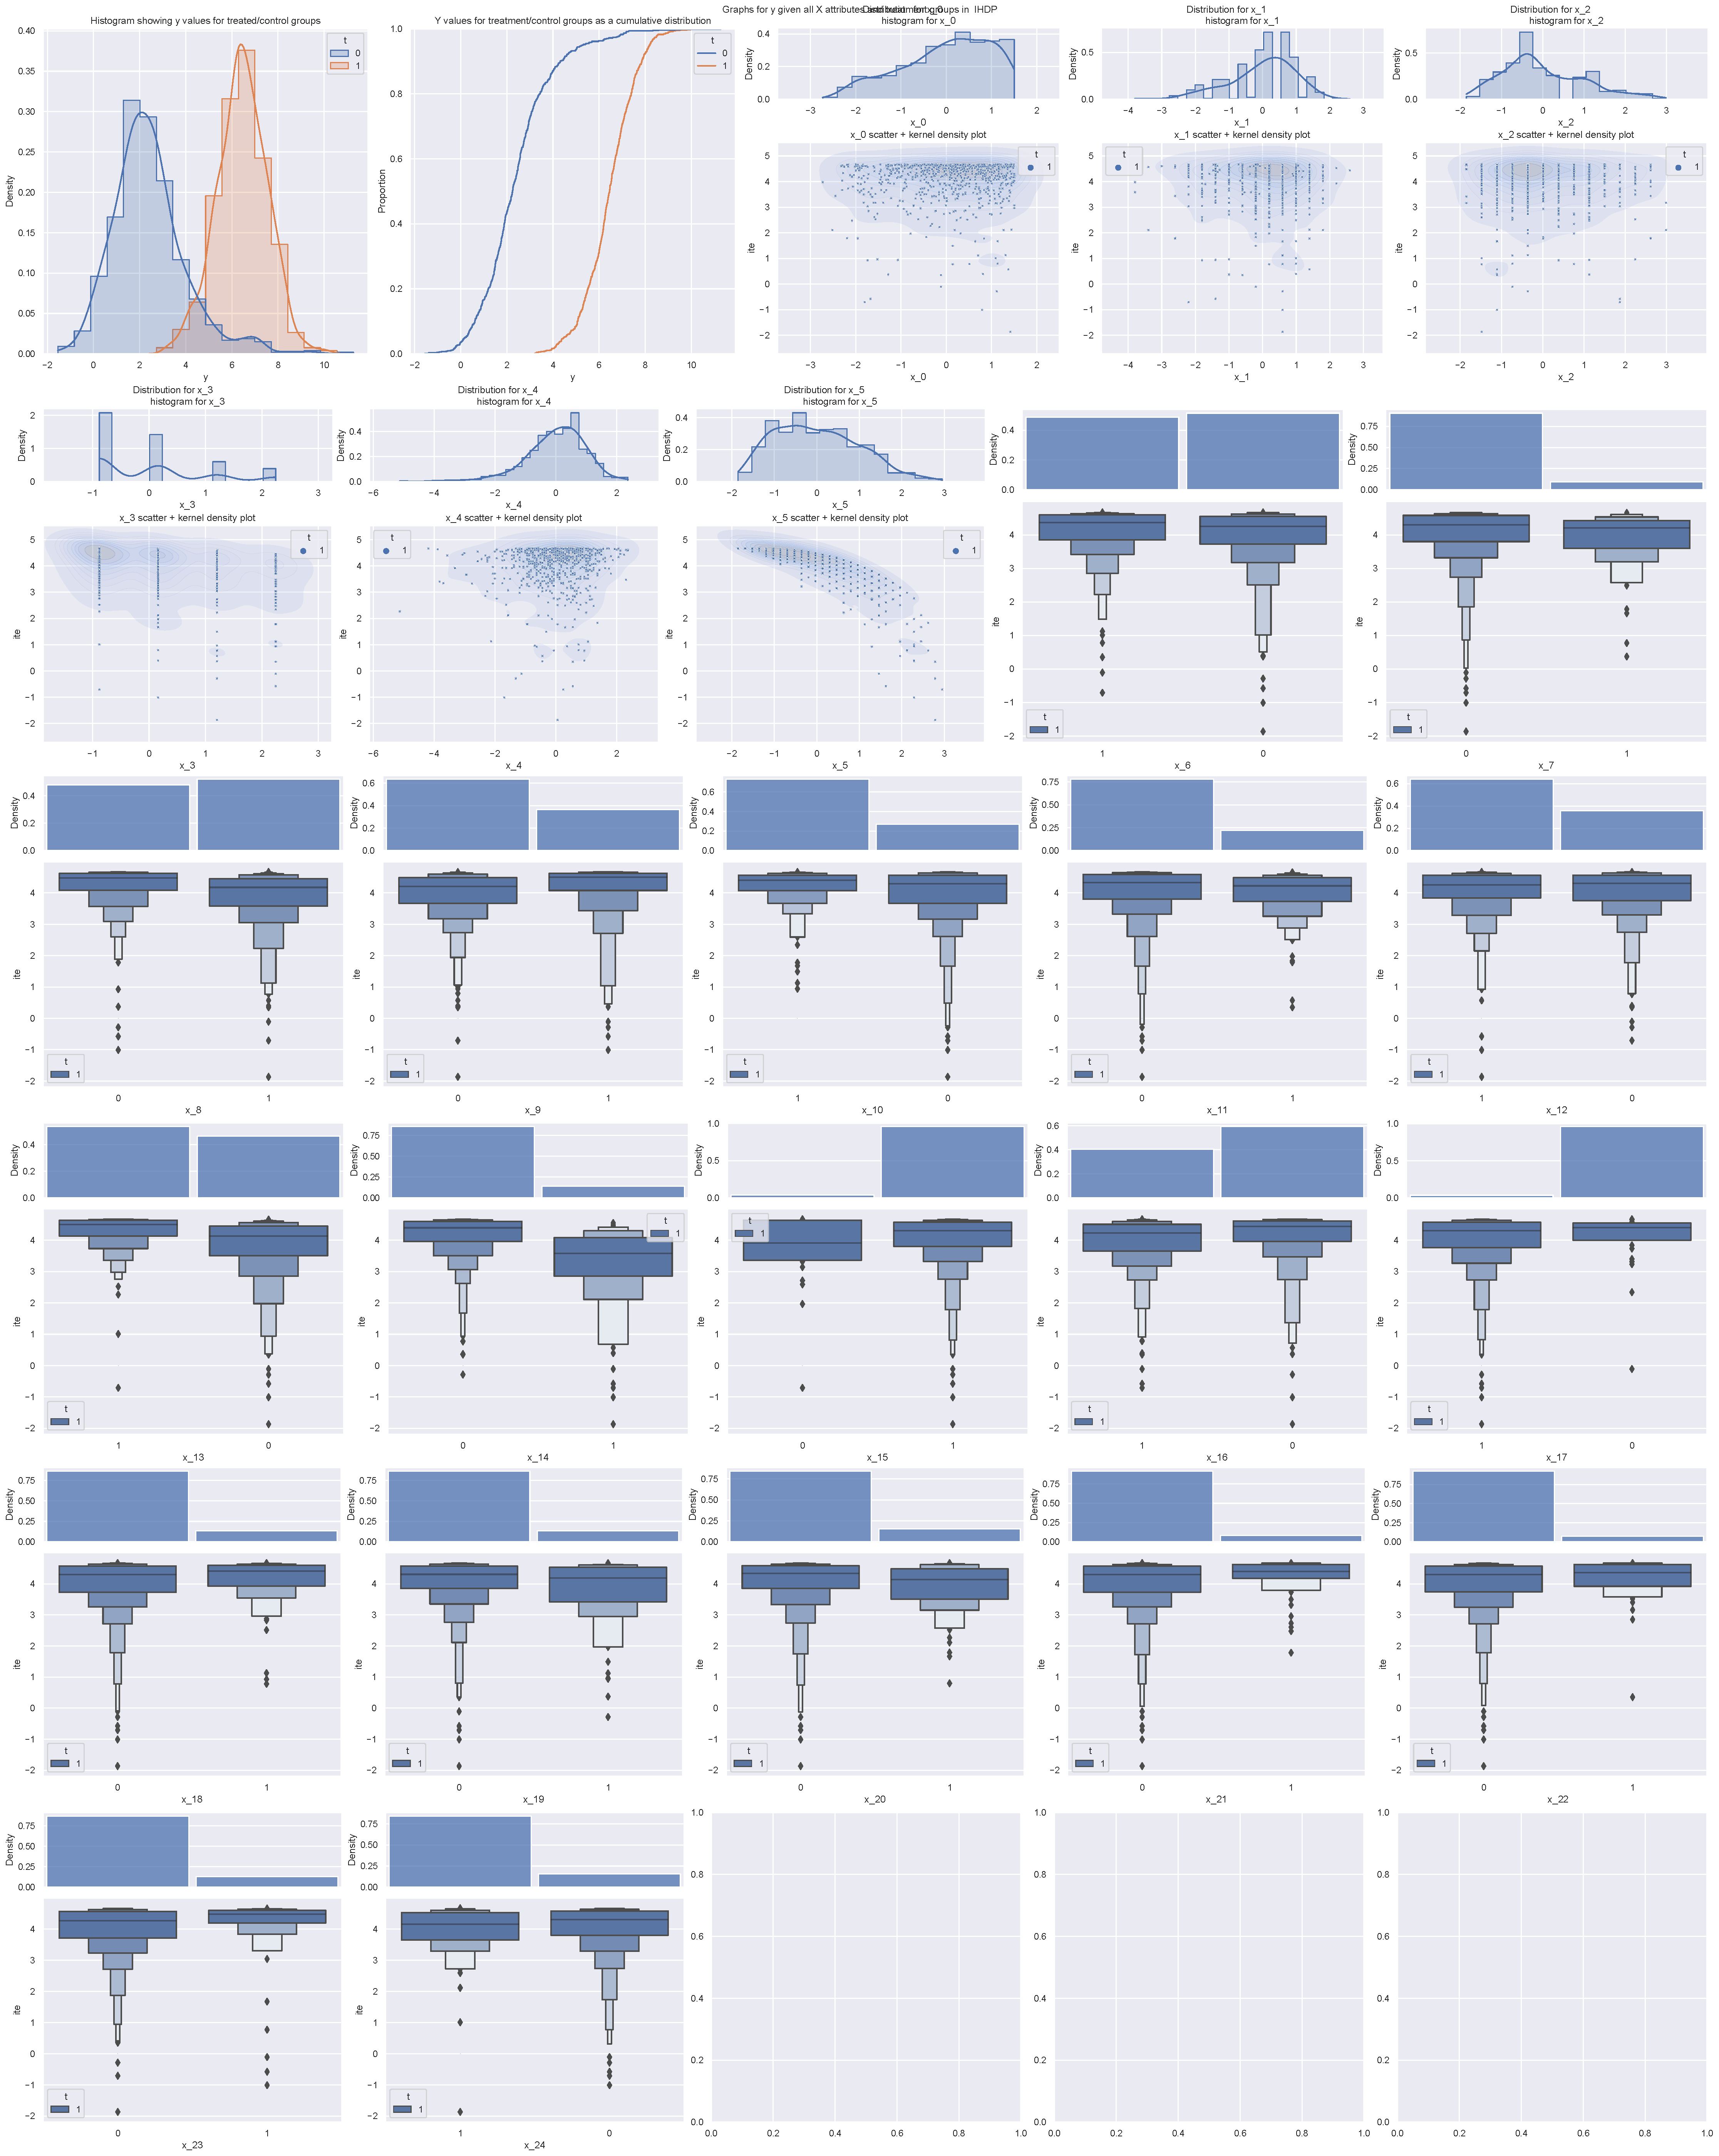
\includegraphics[width=1\textwidth]{project/data/ihdp_graphs.pdf}
    \caption{
        \label{fig:ihdpgraphs}Several graphs for the IHDP dataset, including counterfactuals
    }
\end{figure}

These graphs show how the \texttt{ite} values (along with \texttt{t0} and \texttt{t1})
vary for each individual, based on the value of each \texttt{x} variable for each individual. \texttt{t0}, \texttt{t1}, and \texttt{ite} are based on known counterfactual
data (end result being that \texttt{t0} contains the \texttt{y} value for the case where
the individual was in the control group, and vice versa for \texttt{t1}).

Looking at the density/regression plot between \texttt{t0} and \texttt{t1}, 
we can see a general improvement in the \texttt{y} scores for the population when
receiving the treatment, with few individuals falling below the \texttt{y=x diagonal}
line (these individuals being those who had a negative \texttt{ite}).

We can see a somewhat clear negative correlation between \texttt{x5} and \texttt{ite},
and we can also see that, for several of the binary-valued \texttt{x} values,
there is a rather large imbalance in the quantities of individuals in the dataset
who have each value, which could limit the amount of useful information we could
potentially gain from these variables.

\FloatBarrier

\begin{figure}[H]
    \centering
    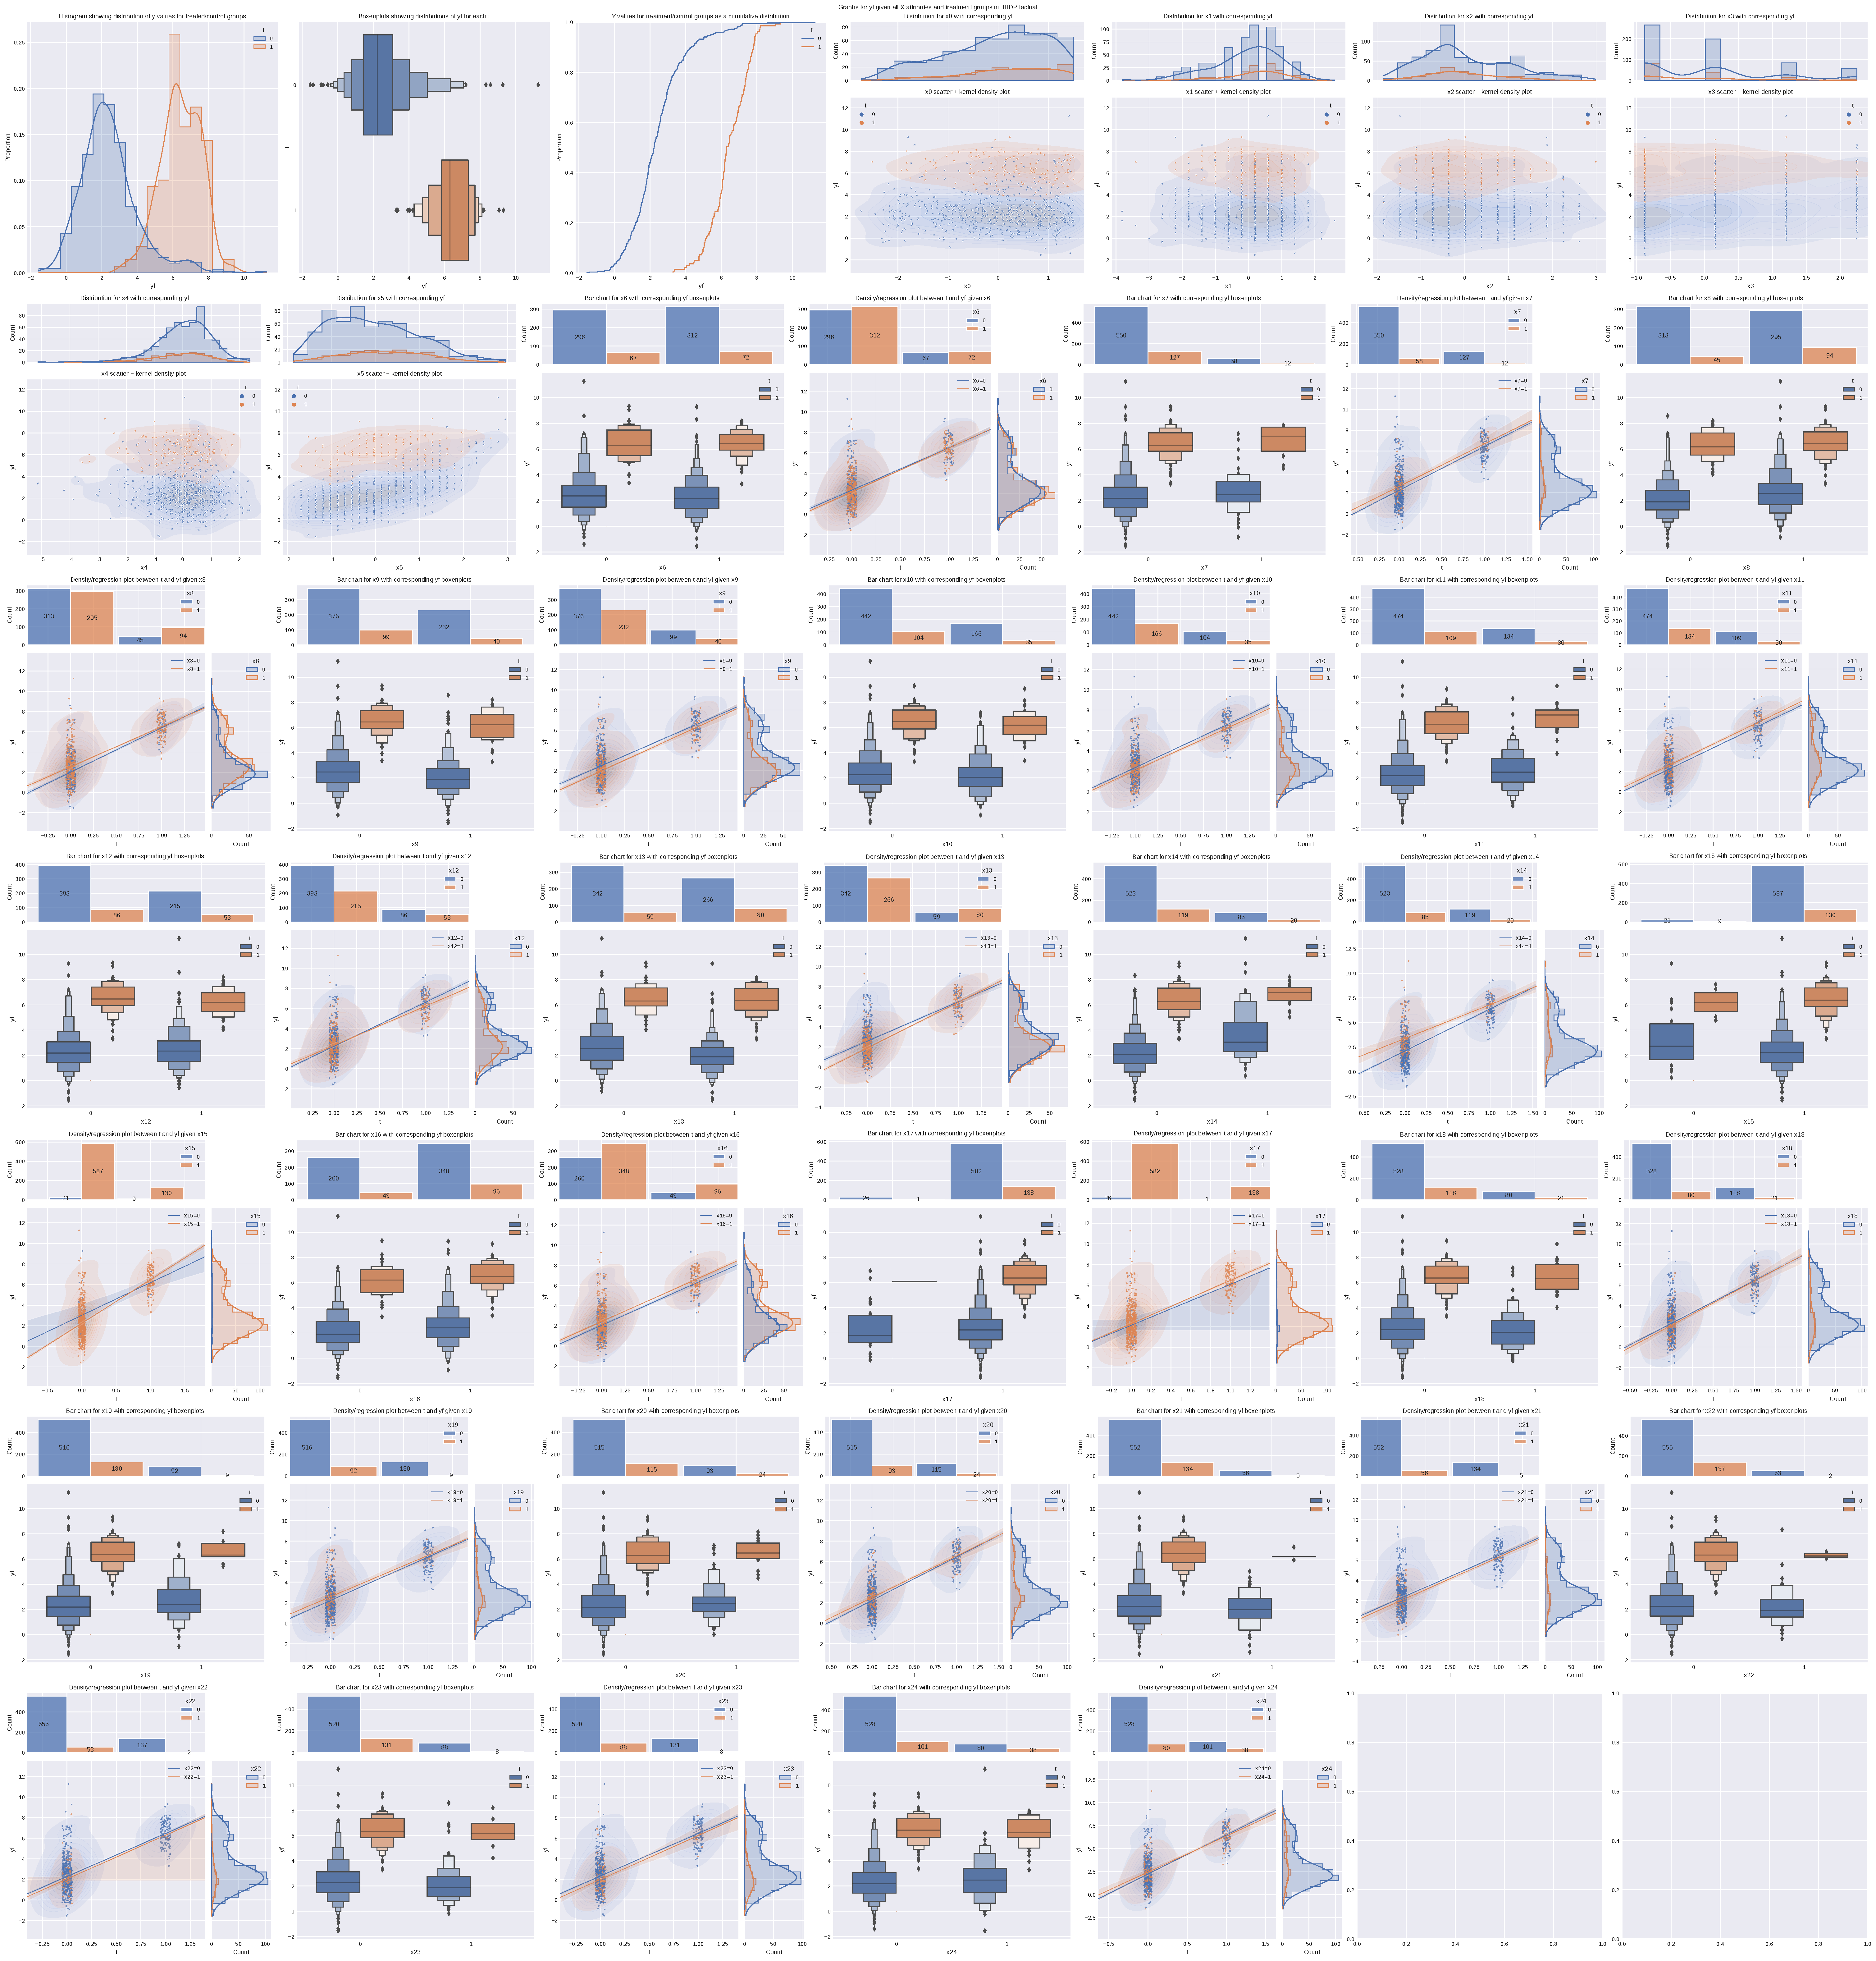
\includegraphics[width=1\textwidth]{project/data/ihdp_factuals.pdf}
    \caption{
        \label{fig:ihdpfact}Graphs for the factual data in IHDP
    }

\end{figure}

These graphs are of the factual data (\texttt{yf}) within the IHDP dataset.
These do illustrate the general positive correlation between individuals receiving
treatment and having a higher \texttt{yf} value, but also shows how imbalanced
this dataset is (most notably with \texttt{x17}, where only 27 individuals have
\texttt{x17==0}.
        
These graphs clearly illustrate that the treated individuals generally have higher
\texttt{yf} values than their untreated peers, with roughly similar interquartile
ranges for treatment/control groups with different values for each binary
\texttt{x} value (even in the extremely unbalanced cases).

\FloatBarrier

\begin{figure}[H]
    \centering
    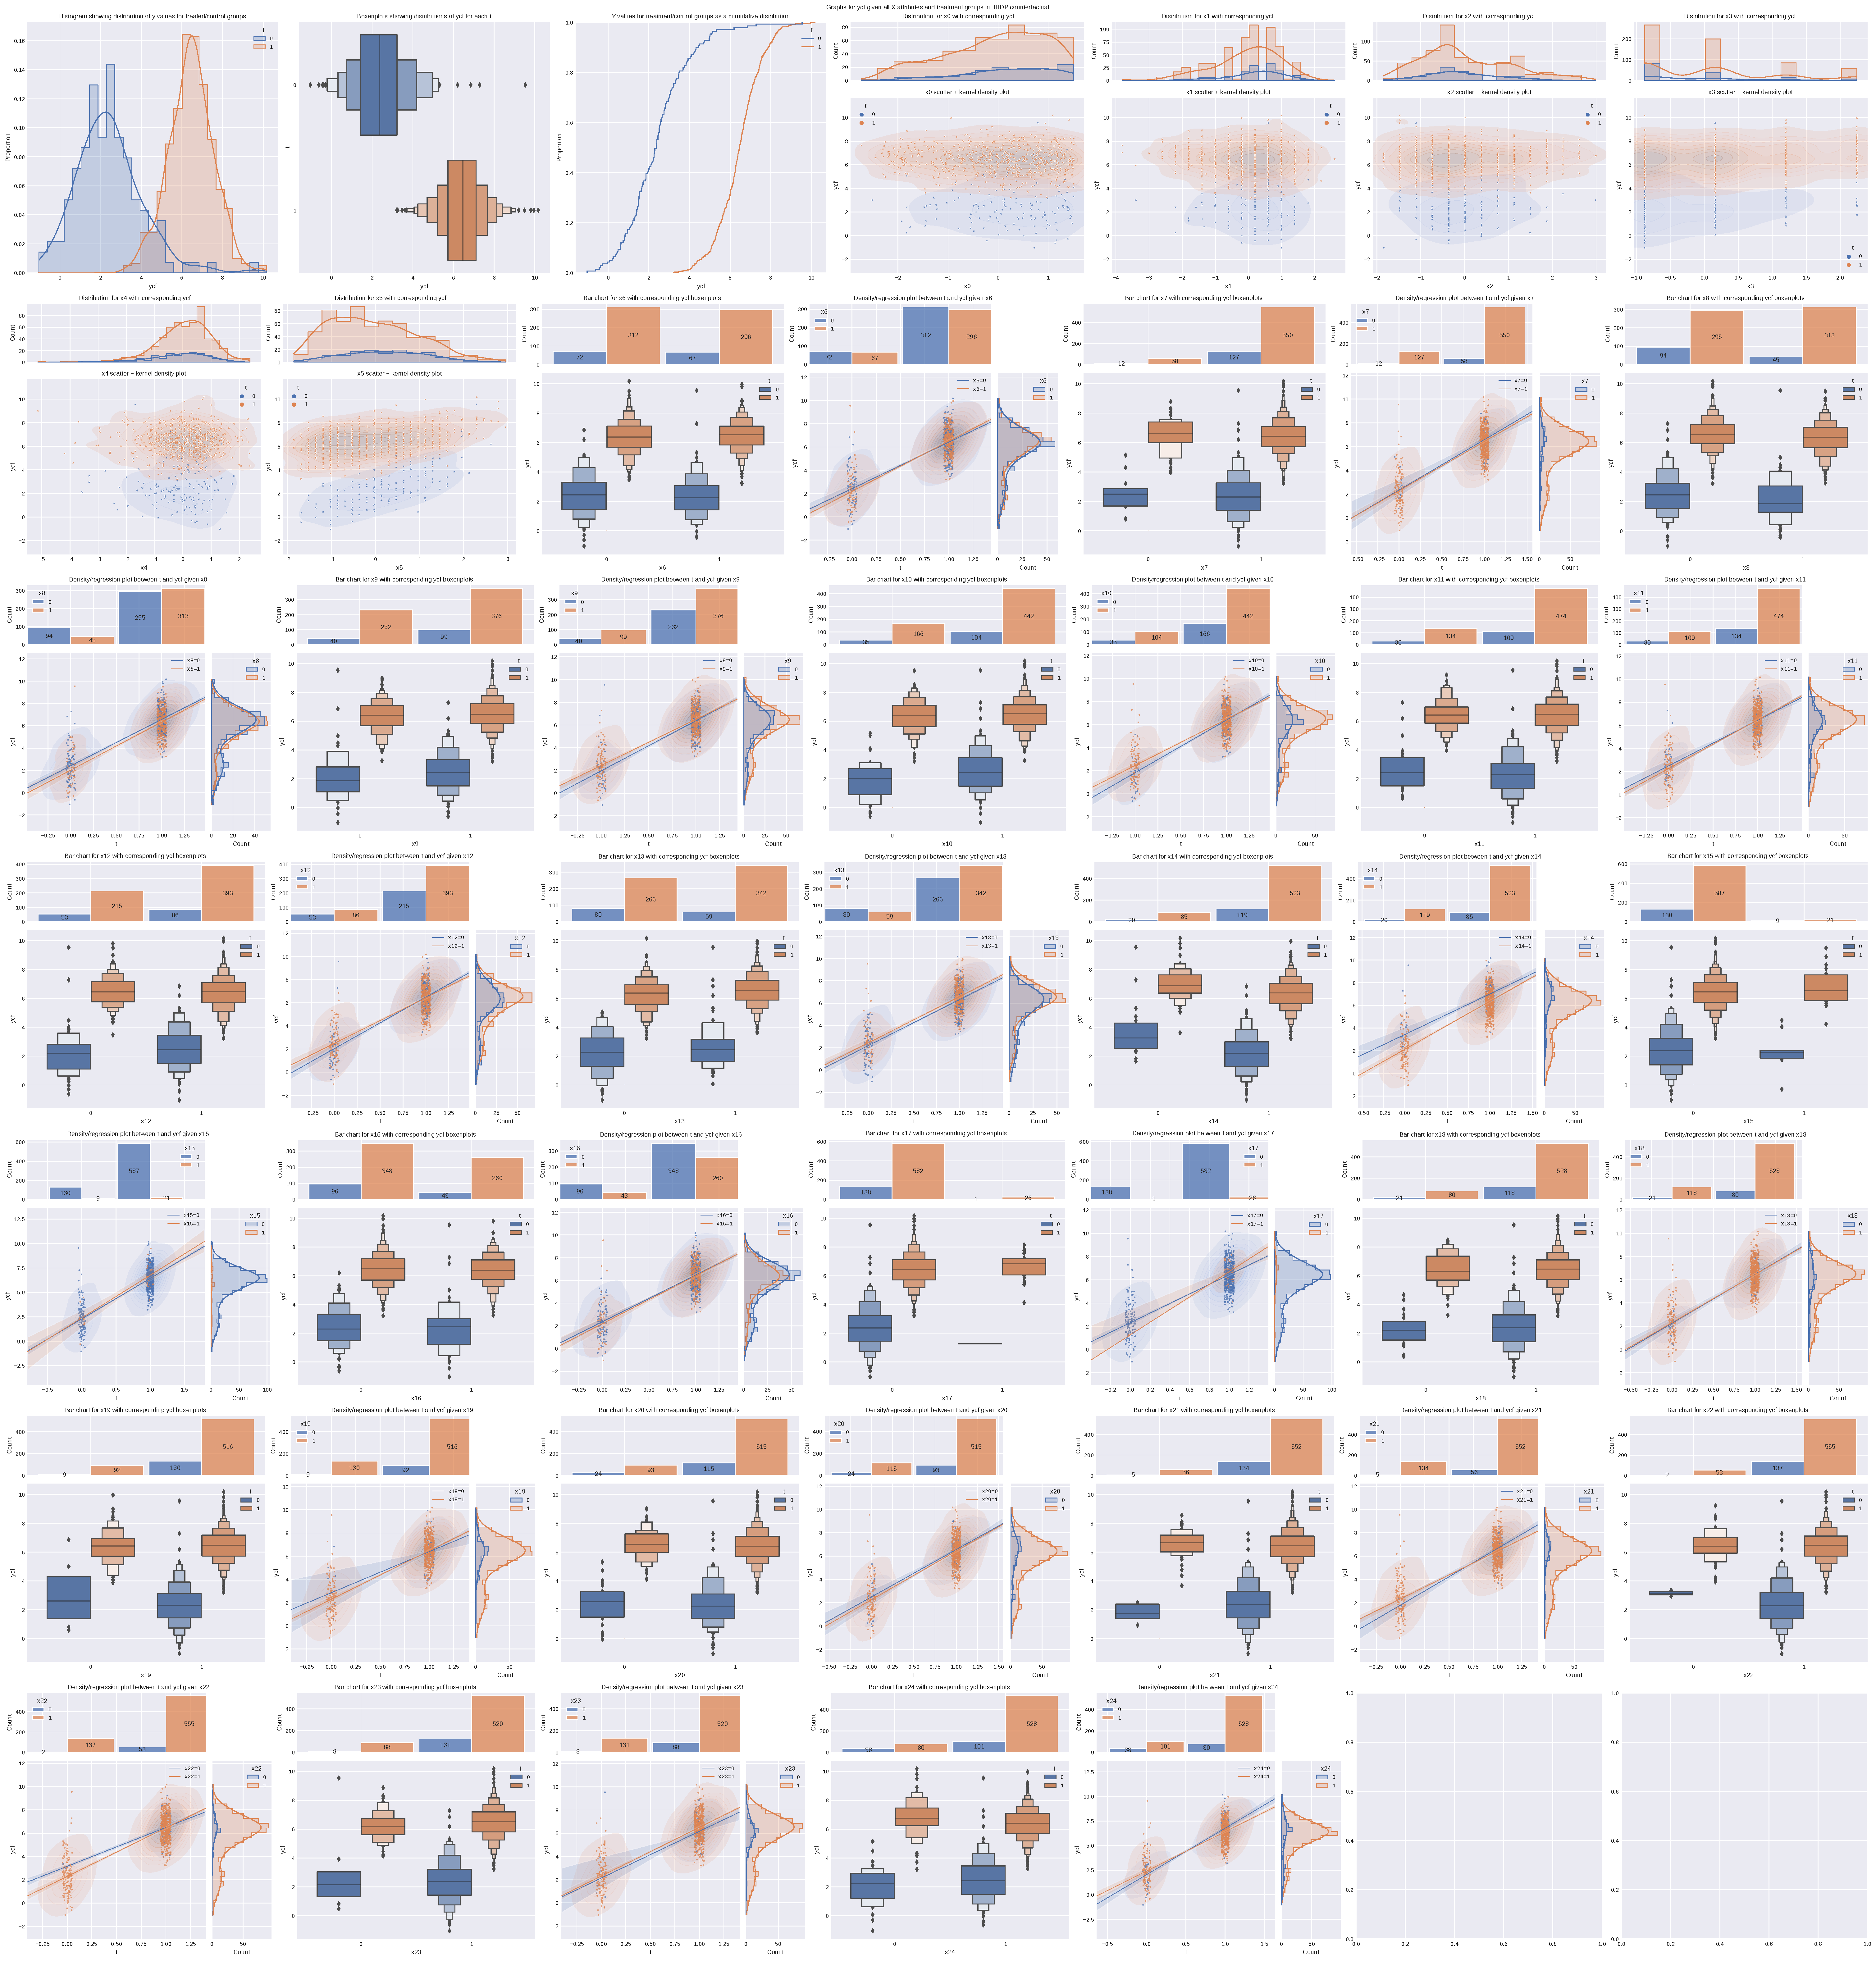
\includegraphics[width=1\textwidth]{project/data/ihdp_counterfactuals.pdf}
    \caption{\label{fig:ihdpcf}Graphs for the counterfactual data in IHDP}
\end{figure}

\FloatBarrier

\subsection{JOBS dataset visualizations}


Here are the graphs for the JOBS dataset.

\FloatBarrier

\begin{figure}[H]
\centering
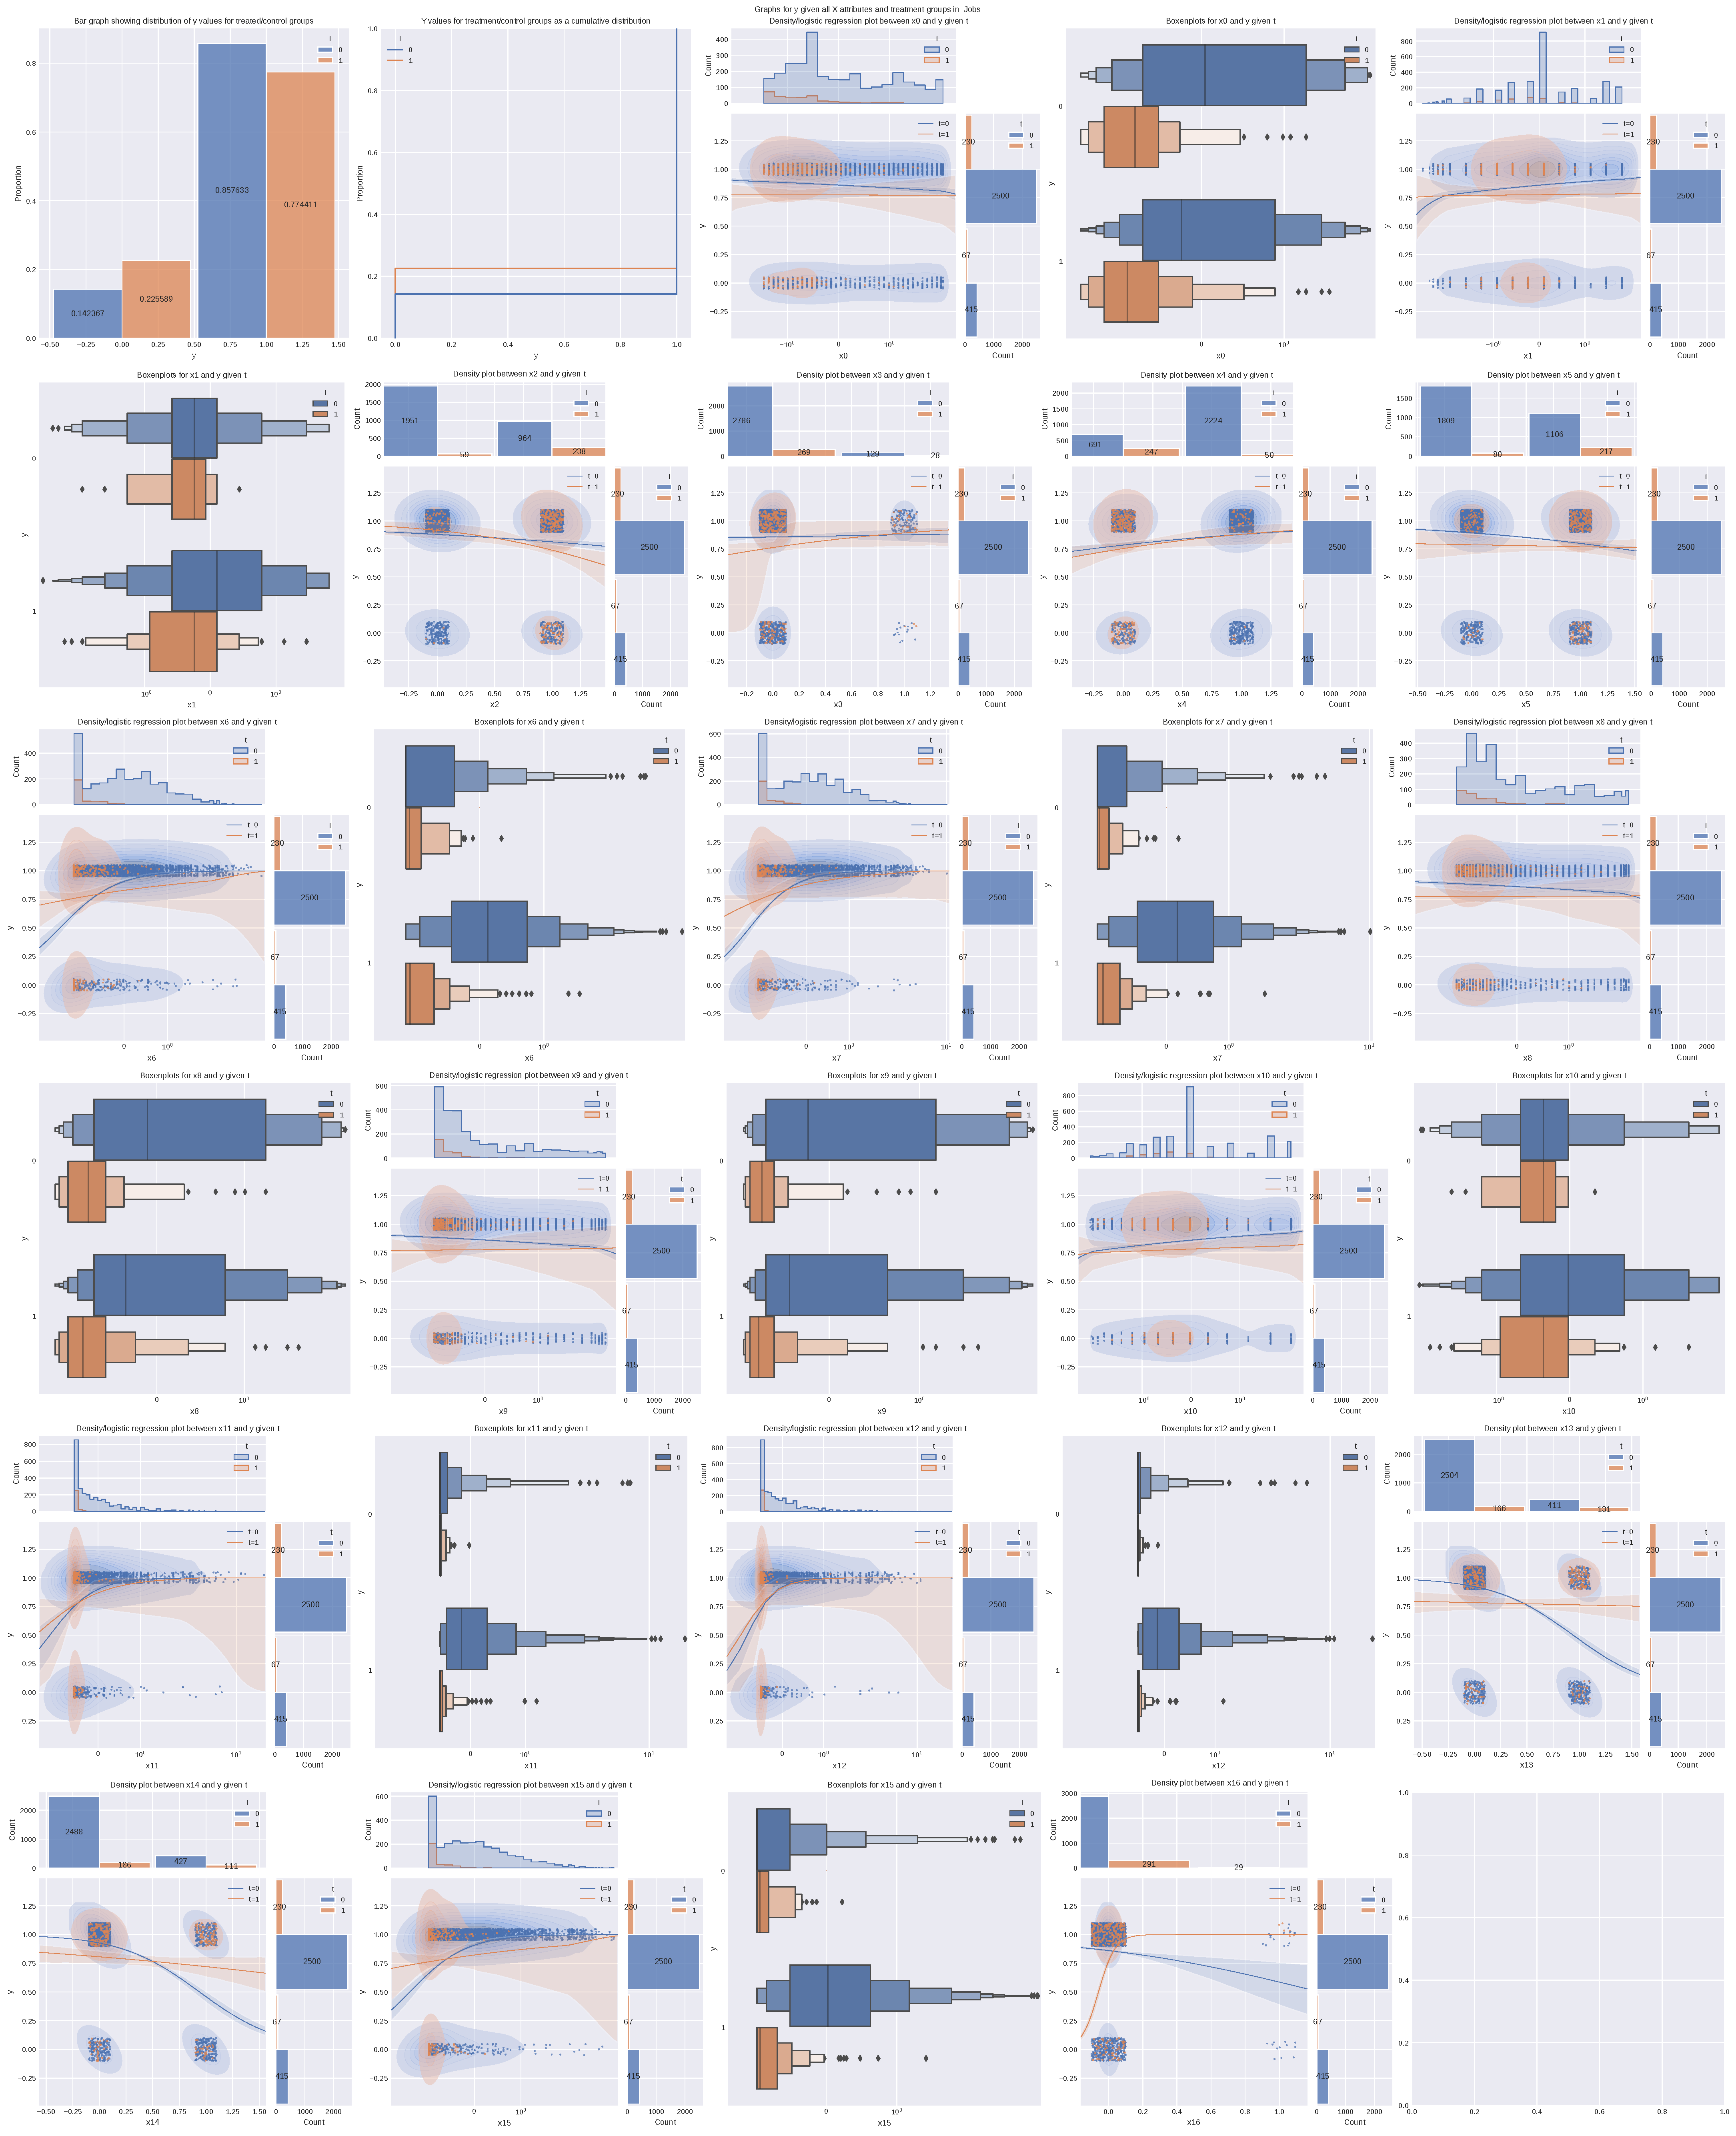
\includegraphics[width=1\textwidth]{project/data/jobs_graphs.pdf}
\caption{\label{fig:jobsgraphs}Several graphs for the JOBS dataset}
\end{figure}

\FloatBarrier

\quoteOFF
\printbibliography


\end{document}